{ %section1_3
	\subsection{Классификация параллельных систем (архитектур)}
	\parПо физической архитектуре параллельные системы можно разделить на 2 типа:
		\begin{enumerate}
			\item\textbf{SMP} (Shared Memory Parallelism, Symmetric MultiProcessor system) – многопроцессорность, многоядерность, GPGPU. 
			\item\textbf{MPP} (Massively Parallel Processing) – кластерные системы, GRID (распределенные вычисления).
		\end{enumerate}
	\parДалее рассмотрим эти две архитектуры подробнее.
	\par\textbf{\textit{SMP}}  - архитектура многопроцессорных систем, в которой два или более одинаковых процессора сравнимой производительности подключаются единообразно к общей памяти (и периферийным устройствам) и выполняют одни и те же функции (почему, собственно, система и называется симметричной). В английском языке SMP-системы носят также название tightly coupled multiprocessors, так как в этом классе систем процессоры тесно связаны друг с другом через общую шину и имеют равный доступ ко всем ресурсам вычислительной системы (памяти и устройствам ввода-вывода) и управляются все одной копией операционной системы. В этой архитектуре все процессоры расположены на одной физической машине, поэтому они имеют общие банки памяти. Существует два вида подключения процессоров к общей памяти:
		\begin{itemize}
			\itemСоединение по общей шине (system bus) изображено на рисунке~\ref{SMPSystemBus:image}. В этом случае только один процессор может обращаться к памяти в каждый данный момент, что накладывает существенное ограничение на количество процессоров, поддерживаемых в таких системах. Чем больше процессоров, тем больше нагрузка на общую шину, тем дольше должен ждать каждый процессор, пока освободится шина, чтобы обратиться к памяти. Снижение общей производительности такой системы с ростом количества процессоров происходит очень быстро, поэтому обычно в таких системах количество процессоров не превышает 2-4. Примером SMP-машин с таким способом соединения процессоров являются любые многопроцессорные серверы начального уровня.
				\begin{figure}[H]
					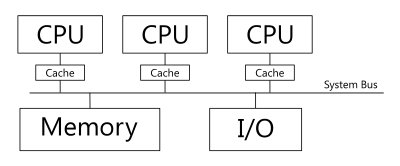
\includegraphics[width=1\linewidth]{SMPSystemBus}
					\caption{\textit{Архитектура SMP. Подключение процессоров по системной шине}}
					\label{SMPSystemBus:image}
				\end{figure}
			\itemКоммутируемое соединение (crossbar switch) изображено на рисунке~\ref{SMPCrossbarSwitch:image}. При таком соединении вся общая память делится на банки памяти, каждый банк памяти имеет свою собственную шину, и процессоры соединены со всеми шинами, имея доступ по ним к любому из банков памяти. Такое соединение схемотехнически более сложное, но оно позволяет процессорам обращаться к общей памяти одновременно. Это позволяет увеличить количество процессоров в системе до 8-16 без заметного снижения общей производительности.
				\begin{figure}[H]
					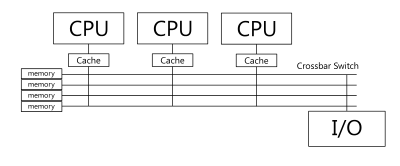
\includegraphics[width=1\linewidth]{SMPCrossbarSwitch}
					\caption{\textit{Архитектура SMP. Подключение процессоров через коммутируемое соединение}}
					\label{SMPCrossbarSwitch:image}
				\end{figure}
		\end{itemize}
	\parПлюсами такого подхода является высокая скорость обмена данными между процессорами и относительная простота в разработке ПО. Однако могут возникнуть проблемы с масштабируемостью системы (если на материнской плате есть только 2 сокета, 3 процессора уже не поставить).
	\par\textbf{\textit{MMP}} - архитектура многопроцессорных систем, при которой память между процессорами разделена физически. На таких системах проводятся распределенные вычисления. Система строится из отдельных узлов, содержащих процессор, локальный банк оперативной памяти, коммуникационные процессоры или сетевые адаптеры, иногда — жёсткие диски и другие устройства ввода-вывода. Доступ к банку оперативной памяти данного узла имеют только процессоры из этого же узла. Узлы соединяются специальными коммуникационными каналами(рисунок~\ref{MMP:image}).
		\begin{figure}[H]
			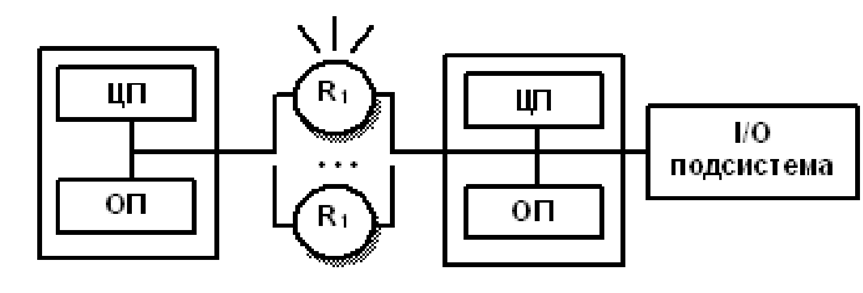
\includegraphics[width=1\linewidth]{MMP}
			\caption{\textit{Архитектура MMP}}
			\label{MMP:image}
		\end{figure}
	\parПлюсами такого подхода является хорошая масштабируемость (при необходимости в увеличении производительности системы достаточно просто добавить еще узлов). Однако существенно понижается скорость межпроцессорного обмена, так как теперь банки памяти разнесены физически. Также стоимость ПО, распределяющее вычисления, очень высока.
	\par
}